\chapter{Implementation}
	\label{chap:implementation}
	
	\section{Tools}
	
	\subsection{Programming Languages}
	
	For the implementation of our application, three primary programming languages deemed to be best suited for development. Apple's Swift programming language \cite{swift} got considered early on, due to the author's familiarisation with the programming language. The programming language gets used for creating applications for Apple's mobile and desktop operating systems, and with 1.5 billion \cite{9to5mac} iOS devices in circulation, that was a lot of potential users. Additionally, Apple's iOS devices are prevalent within most educational settings, with Apple's iPad being one of the primary go-to devices. However, due to the language not supporting key frameworks required, or providing similar alternatives, the decision to not use this language got made. 
	
	We then got presented with three main options to use, \textbf{Python, R and JavaScript} along with HTML and CSS.
	
	Python is a very popular programming language \cite{wired_python, sof_dev_servay20}, it is fast, easy-to-use, and easy-to-deploy programming language that gets widely used to develop scalable applications. Examples include YouTube, Instagram, Pinterest and SurveyMonkey \cite{hackr.io}. The Python Software Foundation state that Python is a high-level object-orientated interpreted language with dynamic semantics. Due to the language being a high-level, it has many built-in data structures. These features, along with the dynamic typing and dynamic binding together make Python attractive to development teams working in a Rapid Application Development (RAD). As Python is an extracted level above the C language \cite{sto_cpython}, Python can get used as the glue that connects existing components, as well as being able to be used as a scripting language \cite{python_desc}. Python gets considered to be easy to learn the language due to its high readability and is recommended by many exam boards as the language to use for teaching Computer Science at GCSE and A-Level level \cite{list exam boards here}. Python's simple and easy to learn syntax emphasises on readability, which, as a result, reduces the cost of program maintenance \cite{python_desc}. 
	
	
	Python gets compared to a lot of other languages. However, due to the requirements and expectations of the application, we will compare it to other similar style applications that can potentially do a similar job. These being Java, JavaScript and C++. In general, the choice of the programming language to use is many other real-world constraints, for example, financial cost, availability, training and even personal preferences and attachments. However, we will focus on language issues for the comparisons.
	
	In comparison to Java, Python programs will typically take 3-5 times quicker (See fig: \ref{fig:py_java_c++}) to develop but will have a slower run time. The time difference gets attributed to Python's built-in data types and its dynamic typing \cite{python_comparison}. As Java gets better characterised as a low-level implementation language, this would be the language of choice if application execution speed was the deciding factor. If this is not a factor, then there is no real benefit over Python.
	
	What gets said about Java is also the same when comparing C++ to Python. It is often 5-10 times shorter than equivalent C++ code! Anecdotal evidence suggests that one Python programmer can finish in two months what two C++ programmers cannot complete in a year. Python shines as a glue language, used to combine components written in C++ \cite{python_comparison}.
	
	In comparison to JavaScript (JS), Python's 'object-based' subset is very similar to JS. Python supports a programming method that uses simple variables and functions, similar to JS, that do not need class definitions. However, Python also supports writing for much larger programs, which leads to more reusable code by using an accurate OOP way while with JS, that is all that it can do \cite{python_comparison}.
	
	
	Another language that presented itself to us was the R language. R is a language and environment for statistical computing and graphics. It is a GNU project which is similar to the S language and environment which was developed at Bell Laboratories (formerly AT\&T, now Lucent Technologies) by John Chambers and colleagues \cite{r_project}. Many users think of R as a statistics system. We prefer to think of it as an environment within which statistical techniques get implemented. R can be extended (easily) via packages \cite{r_project}. Academics and statisticians have developed R over two decades. R has now one of the richest ecosystems to perform data analysis. There are around 12000 packages available in CRAN (open-source repository). It is possible to find a library for whatever the analysis the user wants to perform. The wide variety of library makes R the first choice for statistical analysis, especially for specialised analytical work \cite{r_vs_py}.
	
	R provides a wide variety of statistical (linear and nonlinear modelling, classical statistical tests, time-series analysis, classification, clustering) and graphical techniques, and is highly extensible. One of R's strengths is the ease with which well-designed publication-quality plots can be produced, including mathematical symbols and formulae where needed \cite{r_project}. The cutting-edge difference between R and the other statistical products is the output. R has fantastic tools to communicate the results. Rstudio comes with the library knitr. Xie Yihui wrote this package. He made reporting trivial and elegant. Communicating the findings with a presentation or a document is easy \cite{r_vs_py}.
	
	R is available as Free Software under the terms of the Free Software Foundation's GNU General Public License in source code form. It compiles and runs on a wide variety of UNIX platforms and similar systems (including FreeBSD and Linux), Windows and macOS \cite{r_project}.
	
	R, like S, is designed around a real computer language, and it allows users to add additional functionality by defining new functions. Much of the system is itself written in the R dialect of S, which makes it easy for users to follow the algorithmic choices made. For computationally-intensive tasks, C, C++ and Fortran code can be linked and called at run time. Advanced users can write C code to manipulate R objects directly \cite{r_project}.
		
	\begin{figure}[t]
		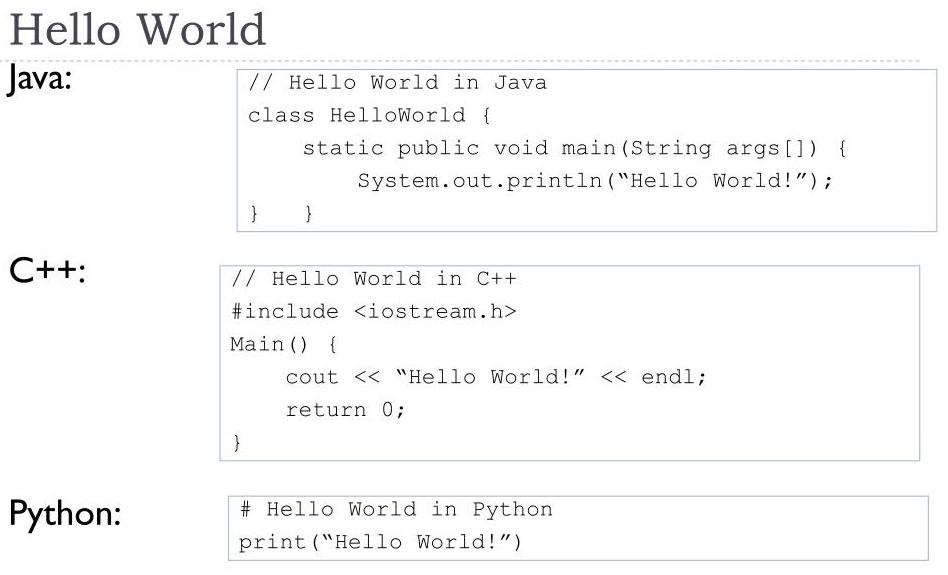
\includegraphics[width=15cm]{graphics/python_vs_java_vs_c++.jpg}
		\caption{A comparison between Java, Python and C++ to print an output to the console. \cite{py_ja_c++}}
		\label{fig:py_java_c++}
	\end{figure}
	
	R and Python are both open-source programming languages with a large community. New libraries or tools are added continuously to their respective catalogue. R is mainly used for statistical analysis, while Python provides a more general approach to data science.
	R and Python are both state of the art in terms of programming language oriented towards data science. Learning both of them is, of course, the ideal solution. R and Python requires a time-investment, and such luxury is not available for everyone. Python is a general-purpose language with a readable syntax. R, however, is built by statisticians and encompasses their specific language \cite{r_vs_py}.
	
	Python can pretty much do the same tasks as R: data wrangling, engineering, feature selection web scrapping, app and so on. Python is a tool to deploy and implement machine learning at a large-scale. Python codes are easier to maintain and more robust than R. Years ago; Python didn't have many data analysis and machine learning libraries. 
	
	Recently, Python is catching up and provides cutting-edge API for machine learning or Artificial Intelligence. Most of the data science job can be done with five Python libraries: Numpy, Pandas, Scipy, Scikit-learn and Seaborn \cite{r_vs_py}.
	
	Python, on the other hand, makes replicability and accessibility easier than R. In fact, if you need to use the results of your analysis in an application or website, Python is the best choice \cite{r_vs_py}.
	
	In 2019 there was an active number of 26.66 billion devices attached to the internet \cite{securitytoday, statista_iot}, with an estimation of 35 billion in 2021 \cite{securitytoday} and by 2025 75.44 billion \cite{statista_iot}. Experts estimate that the IoT device market will reach \$1.1 trillion in 2026 \cite{securitytoday}. Every Second 127 new devices get connected to the world wide web \cite{securitytoday}.
	
	With so many devices on the internet, an important consideration we had was to make the application web-based. By creating the application for the internet, this would allow potentially many more people to be able to access the application and interact with the different ML models. 
	
	In 1989 a British scientist named Sir Tim Berners-Lee started to work on something that would become to be known as the worldwide web (WWW) \cite{web_foundation}. In October of 1990, Tim had created the three fundamental technologies required for the WWW to work\cite{web_foundation}. These were HTML (HyperText Markup Language), which is the markup language for the web, URI (Uniform Resource Identifier), which is the unique address of where the information can get located and HTTP (HyperText Transfer Protocol). The HTTP allows for the retrieval of linked resources from over the www. CSS, on the other hand, was created in 1994 by Håkon Wium Lie at CERN. CSS got created due to believed need that HTML style sheet language for the web, to create "newspaper-like layout in a Web page" \cite{css_history}. These two languages become the cornerstone of web pages. That was, until 1995, where JavaScript got introduced. Whereas HTML and CSS are used to give any website its structure and style, JavaScript is used to to add functionality and different behaviours to a website. It was, therefore, allowing users to interact with the website's content in many imaginative ways.
	
	JS gets regarded as more of the language of the world-wide-web. It got initially designed to be used client-side in a web browser. However, it has in more recent years started to branch out and be able to be used to create applications on, not only the front end of the web but also desktops, servers and mobile platforms natively. For example, React Native, Node.js and TypeScript.
	
	Since the release of JavaScript, it has surpassed Java, Flash, and other languages because it is relatively easy to learn, has a free and open community. JavaScript is also incredibly useful, allowing developers to be able to create apps with audiences in the millions quickly \cite{js_springboard}.
	
	The decision on what language to use we a close call between Python and JavaScript, this was due to the massive amounts of libraries that were on offer and the support communities that were in place. With both being open source and both having essential libraries available to interact with machine learning models and visualisation tools, both could have been a perfect fit for the intended application. However, we decided upon using Python. Python was chosen based on it being the go-to language for anything machine learning related, and its ability to be able to be used multiplatform on desktops or mobile devices. Python supports modules and packages, which encourages programs to be developed modularity and therefore allows code to get reused. The Python interpreter and the extensive standard library are available in source or binary form without charge for all major platforms and can get freely distributed \cite{python_desc}. There was also an additional factor that the author was more familiar with Python and its required libraries compared to the libraries that will get required for using JavaSript.

	There was the additional decision to use HTML and CSS within a small part of the project, the 'Learning Zone', based on the quickness of being able to create and host the webpages containing the learning content. It was allowing the learning content to evolve without having any impact on the overall development of the main application, allowing the learning content to be an individual entity within the main application.
	
	

	
	\section{Frameworks}
	
	\subsection{GUI Framework}
	
	With the nature of the application, we needed to make the application have a Graphical User Interface (GUI). Having a GUI allowed the learning to be a lot more hands-on and allow the players to see what is happening within the models, especially when they interact with them.
	
	Therefore, due to the GUI requirement, three GUI libraries presented themself to us. These were Pygame, PyQT5 and Tkinter.
	
	Pygame is a free, open-sourced library. Released under the LGPL licence, Pygame is a set of Python modules designed for writing video games. Pygame adds functionality on top of the standard Python library. Pygame allows the user to create fully featured games and multimedia programs in the python language \cite{pygame_wiki}.
	
	Pygame is highly portable and runs on nearly every platform and operating system, and it gets downloaded millions of times \cite{pygame_wiki}. 
	
	With the main aim of the application to be a game, Pygame was a strong contender. It was providing modules that can handle a lot of the key gaming mechanics and multiple screen switching. However, it lacked some key features that were deemed essential for the application. It was unable to provide a library that could create interactable graphs to be used as data inputs for the models and be able to render HTML and CSS content for the Learning Zone. Therefore reducing the amount of flexibility, it got decided upon for using HTML and CSS for the learning content. Therefore, meaning that all the content would need to be hardcoded. If any changes were needed, a significant transformation would need to happen to the overall code, instead of just changing the web content.
	
	PyQt is a set of Python v2 and v3 bindings for The Qt Company's Qt application framework and runs on all platforms supported by Qt including Windows, macOS, Linux, iOS and Android. PyQt5 supports Qt v5. PyQt4 supports Qt v4 and will build against Qt v5. The bindings are implemented as a set of Python modules and contain over 1,000 classes \cite{pyqt_rbc}.
	
	PyQt brings together the Qt C++ cross-platform application framework and the cross-platform interpreted language Python.
	Qt is more than a GUI toolkit. It includes abstractions of network sockets, threads, Unicode, regular expressions, SQL databases, SVG, OpenGL, XML, a fully functional web browser, a help system, a multimedia framework, as well as a rich collection of GUI widgets.
	Qt classes employ a signal/slot mechanism for communicating between objects that is type safe but loosely coupled making it easy to create re-usable software components \cite{pyqt_rbc}.
	
	Qt also includes Qt Designer, a graphical user interface designer. PyQt is able to generate Python code from Qt Designer. It is also possible to add new GUI controls written in Python to Qt Designer \cite{pyqt_rbc}.
	
	PyQt combines all the advantages of Qt and Python. A programmer has all the power of Qt but can exploit it with the simplicity of Python \cite{pyqt_rbc}.
	
	Tkinter is the third option. Tkinter commonly comes bundled with Python, using Tk and is Python's standard GUI framework. It is famous for its simplicity and graphical user interface. It is open-source and available under the Python License \cite{data_camp_gui}.
	
	Tkinter is Python's de-facto standard GUI (Graphical User Interface) package. It is a thin object-oriented layer on top of Tcl/Tk.
	Tkinter is not the only GuiProgramming toolkit for Python. It is however the most commonly used one. CameronLaird calls the yearly decision to keep TkInter "one of the minor traditions of the Python world \cite{py_tkinter}."
	
	Tkinter supports functionality with Matplotlib, with Matplotlib offering libraries to allow handling the backend of the graph creation interacting with the GUI library. However, unlike QT, Tkinter does not support any GUI designer. Therefore the GUIs will have to be created programmatically, which will give more control, might involve more of a learning curve and potentially more time to implement in the initial stages.
	
	After reviewing the different GUI libraries, PyQt was the decided library to use. We believed it would give us the ability to have 
	
	
	\section{Packages Used}
	\label{sec:packages_used}
	
	
	\section{IDE Used}
	\label{sec:ide_used}
	
	Pycharm
	
	PyCharm is a dedicated Python Integrated Development Environment (IDE) providing a wide range of essential tools for Python developers, tightly integrated to create a convenient environment for productive Python, web, and data science development \cite{pycharm_get_started}.
	
	VS Code
	
	Visual Studio Code is a free source-code editor made by Microsoft for Windows, Linux and macOS. Features include support for debugging, syntax highlighting, intelligent code completion, snippets, code refactoring, and embedded Git. Visual Studio Code combines the simplicity of a source code editor with powerful developer tooling, like IntelliSense code completion and debugging. First and foremost, it is an editor that gets out of your way. The delightfully frictionless edit-build-debug cycle means less time fiddling with your environment, and more time executing on your ideas \cite{vs_code}.
	
	At its heart, Visual Studio Code features a lightning fast source code editor, perfect for day-to-day use. With support for hundreds of languages, VS Code helps you be instantly productive with syntax highlighting, bracket-matching, auto-indentation, box-selection, snippets, and more. Intuitive keyboard shortcuts, easy customisation and community-contributed keyboard shortcut mappings let you navigate your code with ease.
	
	For serious coding, you'll often benefit from tools with more code understanding than just blocks of text. Visual Studio Code includes built-in support for IntelliSense code completion, rich semantic code understanding and navigation, and code refactoring.
	
	And when the coding gets tough, the tough get debugging. Debugging is often the one feature that developers miss most in a leaner coding experience, so we made it happen. Visual Studio Code includes an interactive debugger, so you can step through source code, inspect variables, view call stacks, and execute commands in the console.
	VS Code also integrates with build and scripting tools to perform common tasks making everyday workflows faster. VS Code has support for Git so you can work with source control without leaving the editor including viewing pending changes diffs \cite{vs_code}..
	
	Customise every feature to your liking and install any number of third-party extensions. While most scenarios work "out of the box" with no configuration, VS Code also grows with you, and we encourage you to optimise your experience to suit your unique needs. VS Code is an open-source project so you can also contribute to the growing and vibrant community on GitHub.
	
	
	Atom
	
	Atom was developed and released by GitHub. This free, open-source code editor is self-labeled 'a hackable text editor for the 21st century'. And hackable, it is. Atom allows developers to fully customise the look, feel, and requirements to speed up their workflows.
	However, Atom still allows developers to use it productively without ever touching a config file. A freshly downloaded version comes pre-loaded with eight syntax themes and four UI: two light and two dark. But, if none of the pre-installed themes interest you, Atom makes it easy and quick to install customised themes created by a third-party or to create one yourself \cite{atom_explain}.
	
	
	Chosen IDE
	VS Code -  Due to familiarity and Extension features
	
	
	\section{Intricacies of the Game Components}
	\label{sec:packages_used}
	
	\subsection{Gameplay Area}
	
	\subsection{Free Play Area}
	
	\subsection{Learning Zone Area}
	
	\subsection{Achievements Area}
	
	
	\section{Example user stories (A UML term for case studies or example playthroughs)}
	\label{sec:ide_used}
	
	
	
